\documentclass[conference]{IEEEtran}
\usepackage[utf8]{inputenc}
\usepackage[T1]{fontenc}
\usepackage[portuguese]{babel}

\usepackage{float} 
\usepackage{url}  
\usepackage{multirow}
\usepackage{caption}
\usepackage{subcaption}
\usepackage{booktabs}
\usepackage{cite}
\pagestyle{plain}
\usepackage{amsmath}
\usepackage{float}
\usepackage{tikz}
\usepackage{placeins}
\usepackage{comment}
\usepackage{tabularx}
\usepackage{algorithm}
\usepackage{algpseudocode}
\usepackage{graphicx}
\floatname{algorithm}{Algoritmo}
\ifCLASSINFOpdf
  \usepackage[pdftex]{graphicx}
\fi

\hyphenation{op-tical net-works semi-conduc-tor}

\begin{document}

%selection sort, insertion sort, quick sort(LR PTRS), merge sort, heap sort, radix sort (LSD e MSD), std sort gcc, std::stable_sort gcc, shell sort, cocktail shaker, gnome sort, bitonic sort, bogo sort
\title{algortimos de ordenacao ? referencias}

\author{\IEEEauthorblockN{\\ Hugo Veríssimo}
\IEEEauthorblockA{Optimização Combinatória 24/25\\
Universidade de Aveiro\\
Aveiro, Portugal\\
hugoverissimo@ua.pt}
\and
\IEEEauthorblockN{\\ João Cardoso}
\IEEEauthorblockA{Optimização Combinatória 24/25\\
Universidade de Aveiro\\
Aveiro, Portugal\\
joaopcardoso@ua.pt}}

\maketitle
\thispagestyle{plain}

\begin{abstract}
cona cona caon
\end{abstract}

\begin{quote}
\small
\noindent
\textbf{Palavras-chave:} zzz, aaa
\end{quote}

\IEEEpeerreviewmaketitle

\section{Introdução}

Os algoritmos de ordenação são essenciais em várias áreas da optimização combinatória e da investigação operacional, sendo utilizados para organizar dados de forma eficiente, melhorar o desempenho de algoritmos de procura e reduzir a complexidade computacional de problemas em larga escala.

Em contextos de otimização combinatória, onde para vários problemas se torna fundamental a ordenação prévia de dados, como nas heurísticas para o problema Knapsack, no algoritmo de Kruskal para construção de árvores geradoras mínimas, ou em algoritmos gulosos para cobertura de conjuntos, a escolha do método de ordenação pode impactar significativamente a eficiência global da solução.

% POR MELHORAR ESTE PARÁGRAFO
Este trabalho visa explorar os principais algoritmos de ordenação, destacando as suas características, o seu funcionamento, a complexidade computacional associada e uma análise comparativa entre os mesmos. Considerando as diferentes implementações e constrangimentos associados, exploramos os cenários onde cada algoritmo poderá ser mais útil. 
%SERÃO ABORDADOS ALGORITMOS COMO O QUICKSORT, .........
O objetivo é compreender como a ordenação pode ser utilizada de forma estratégica para melhorar a eficiência de algoritmos em diversos cenários, e como otimizações na própria ordenação podem levar a avanços significativos em problemas computacionalmente intensivos.

% Like insertion sort, bubble sort is adaptive, which can give it an advantage over algorithms like quicksort. This means that it may outperform those algorithms in cases where the list is already mostly sorted (having a small number of inversions), despite the fact that it has worse average-case time complexity. For example, bubble sort is O ( n ) {\displaystyle O(n)} on a list that is already sorted, while quicksort would still perform its entire O ( n log ⁡ n ) {\displaystyle O(n\log n)} sorting process. Útil para discutir os resultados, e potencial utilidade

\section{Algoritmos de Ordenação}

Nesta secção serão apresentados os algoritmos selecionados, detalhando-se individualmente o seu princípio básico de funcionamento, a complexidade temporal, as vantagens e desvantagens, e a aplicabilidade prática em diferentes cenários da otimização combinatória. POR REVER SE REALMENTE SE FAZ ISTO TUDO E MUDAR ?!?!?!??!

\subsection{Bubble Sort acrescentar informação sobre a família Exchange sorts}

O algoritmo \textit{Bubble sort} consiste em comparar um dado item com todos os elementos de uma lista, em que o item vai se reposicionando com elementos comparativamente menores até encontrar um item maior ou chegar ao fim da lista. O nome do algoritmo prende-se com a forma como o elemento comparado vai ascendendo (ou afundando, consoante seja usado), tal como uma bolha na água. 

Tipicamente este algoritmo não encontra aplicação em casos reais devido à sua ineficiência e complexidade de ordem \(O(n^2)\). No entanto, a sua rápida implementação pode ser de interesse em casos particulares, em que listas que estejam próximas da sua forma ordenada passam pelo algoritmo com uma complexidade de ordem \(O(n)\).

\begin{algorithm}[H]
    \raggedright
    \vspace{.1em}
    \textbf{Entrada:} lista \textit{arr} \\
    \textbf{Saída:} lista ordenada \textit{arr} \\
    \vspace{.5em}
    \hrule 
    \caption{Bubble Sort}
    \begin{algorithmic}[1]
        \State $n \gets$ \text{len}$(arr)$
        
        \For{$i$ from $0$ to $n - 1$}
            \State $swapped \gets$ False
            \For{$j$ from $0$ to $n - 2 - i$}
                \If{$arr[j] > arr[j+1]$}
                    \State Swap $arr[j]$ and $arr[j+1]$
                    \State $swapped \gets$ True
                \EndIf
            \EndFor
            \If{not $swapped$}
                \State \textbf{break}
            \EndIf
        \EndFor
    
        \State \Return $arr$
    \end{algorithmic}
\end{algorithm}

FALAR DA COMPLEXIDADE DO ALGORITMO A PARTIR DA ANÁLISE DO MESMO

Existem algoritmos baseados nesta abordagem, tal como o \textit{Cocktail sort}, que aplica a metodologia em sentido crescente e decrescente, tornando-o mais rápido por norma, mas com o mesmo grau de complexidade no pior cenário.

\subsection{Selection Sort}

O algoritmo de \textit{Selection sort} tem um procedimento bastante diferente do algoritmo anterior. Faz parte da família de algoritmos de \textit{Selection sorts}, em que a lista de items ordenados vai sendo gerada por comparação a partir da lista original desordenada. No algoritmo em questão, procura-se o menor elemento disponível e coloca-se no início da nova lista. Estes passos repetem-se na lista desordenada até não existirem mais e a lista ordenada ser criada.

\begin{algorithm}[H]
    \raggedright
    \vspace{.1em}
    \textbf{Entrada:} lista \textit{arr} \\
    \textbf{Saída:} lista ordenada \textit{arr} \\
    \vspace{.5em}
    \hrule 
    \caption{Selection Sort}
    \begin{algorithmic}[1]
        \State $n \gets$ \text{len}$(arr)$
    
        \For{$i$ from $0$ to $n - 1$}
            \State $min\_idx \gets i$
            \For{$j$ from $i + 1$ to $n - 1$}
                \If{$arr[j] < arr[min\_idx]$}
                    \State $min\_idx \gets j$
                \EndIf
            \EndFor
            \If{$min\_idx \neq i$}
                \State Swap $arr[i]$ and $arr[min\_idx]$
            \EndIf
        \EndFor
    
        \State \Return $arr$
    \end{algorithmic}
\end{algorithm}

FALAR DA COMPLEXIDADE DO ALGORITMO A PARTIR DA ANÁLISE DO MESMO

Dentro desta família de algoritmos, há um que devemos destacar, chamado \textit{Gnome sort},  que consiste nas operações do \textit{Selection sort}, mas sem ter o segundo ciclo dentro do primeiro, resultando num número de operações semelhante ao \textit{Insertion sort}, e por consequência pior que o \textit{Selection sort}.

\subsection{Insertion Sort}

\begin{algorithm}[H]
    \raggedright
    \vspace{.1em}
    \textbf{Entrada:} lista \textit{arr} \\
    \textbf{Saída:} lista ordenada \textit{arr} \\
    \vspace{.5em}
    \hrule 
    \caption{Insertion Sort}
    \begin{algorithmic}[1]
        \For{$i$ from $1$ to $\text{len}(arr) - 1$}
            \State $key \gets arr[i]$
            \State $j \gets i - 1$
            \While{$j \geq 0$ and $arr[j] > key$}
                \State $arr[j + 1] \gets arr[j]$
                \State $j \gets j - 1$
            \EndWhile
            \State $arr[j + 1] \gets key$
        \EndFor
    
        \State \Return $arr$
    \end{algorithmic}
\end{algorithm}

FALAR DA COMPLEXIDADE DO ALGORITMO A PARTIR DA ANÁLISE DO MESMO

\subsection{Counting Sort}

\begin{algorithm}[H]
    \raggedright
    \vspace{.1em}
    \textbf{Entrada:} lista \textit{arr} \\
    \textbf{Saída:} lista ordenada \textit{sorted\_arr} \\
    \vspace{.5em}
    \hrule 
    \caption{Counting Sort}
    \begin{algorithmic}[1]
        \State $max\_val \gets \max(arr)$
        \State $count \gets$ array of zeros with length $max\_val + 1$
        
        \For{each $num$ in $arr$}
            \State $count[num] \gets count[num] + 1$
        \EndFor
    
        \State $sorted\_arr \gets$ empty list
        \For{$i$ from $0$ to $max\_val$}
            \If{$count[i] > 0$}
                \State Append $count[i]$ copies of $i$ to $sorted\_arr$
            \EndIf
        \EndFor
    
        \State \Return $sorted\_arr$
    \end{algorithmic}
\end{algorithm}

FALAR DA COMPLEXIDADE DO ALGORITMO A PARTIR DA ANÁLISE DO MESMO

\subsection{Radix Sort}

\begin{algorithm}[H]
    \raggedright
    \vspace{.1em}
    \textbf{Entrada:} lista \textit{arr} \\
    \textbf{Saída:} lista ordenada \textit{arr} \\
    \vspace{.5em}
    \hrule 
    \caption{Radix Sort}
    \begin{algorithmic}[1]
        \Function{CountingSortRadix}{$arr$, $exp$}
            \State $n \gets$ \text{len}$(arr)$
            \State $output \gets$ array of zeros of length $n$
            \State $count \gets$ array of zeros of length $10$
    
            \For{$i$ from $0$ to $n - 1$}
                \State $index \gets (arr[i] \div exp) \bmod 10$
                \State $count[index] \gets count[index] + 1$
            \EndFor
    
            \For{$i$ from $1$ to $9$}
                \State $count[i] \gets count[i] + count[i - 1]$
            \EndFor
    
            \For{$i$ from $n - 1$ to $0$}
                \State $index \gets (arr[i] \div exp) \bmod 10$
                \State $output[count[index] - 1] \gets arr[i]$
                \State $count[index] \gets count[index] - 1$
            \EndFor
    
            \For{$i$ from $0$ to $n - 1$}
                \State $arr[i] \gets output[i]$
            \EndFor
        \EndFunction
    
        \State $max\_num \gets \max(arr)$
        \State $exp \gets 1$
        \While{$max\_num \div exp > 0$}
            \State \Call{CountingSortRadix}{$arr$, $exp$}
            \State $exp \gets exp \times 10$
        \EndWhile
    
        \State \Return $arr$
    \end{algorithmic}
\end{algorithm}

FALAR DA COMPLEXIDADE DO ALGORITMO A PARTIR DA ANÁLISE DO MESMO

\subsection{Quick Sort}

\begin{algorithm}[H]
    \raggedright
    \vspace{.1em}
    \textbf{Entrada:} lista \textit{arr} \\
    \textbf{Saída:} lista ordenada \textit{arr} \\
    \vspace{.5em}
    \hrule 
    \caption{Quick Sort}
    \begin{algorithmic}[1]
        \Function{Partition}{$items$, $low$, $high$}
            \State $pivot \gets items[high]$
            \State $i \gets low - 1$
            \For{$j$ from $low$ to $high - 1$}
                \If{$items[j] \leq pivot$}
                    \State $i \gets i + 1$
                    \State Swap $items[i]$ and $items[j]$
                \EndIf
            \EndFor
            \State Swap $items[i + 1]$ and $items[high]$
            \State \Return $i + 1$
        \EndFunction
    
        \Function{QuickSort}{$items$, $low$, $high$}
            \If{$low < high$}
                \State $pivot\_index \gets$ \Call{Partition}{$items$, $low$, $high$}
                \State \Call{QuickSort}{$items$, $low$, $pivot\_index - 1$}
                \State \Call{QuickSort}{$items$, $pivot\_index + 1$, $high$}
            \EndIf
        \EndFunction
    
        \State \Call{QuickSort}{$arr$, $0$, $\text{len}(arr) - 1$}
        \State \Return $arr$
    \end{algorithmic}
\end{algorithm}

FALAR DA COMPLEXIDADE DO ALGORITMO A PARTIR DA ANÁLISE DO MESMO

\subsection{Merge Sort}

\begin{algorithm}[H]
    \raggedright
    \vspace{.1em}
    \textbf{Entrada:} lista \textit{arr} \\
    \textbf{Saída:} lista ordenada \textit{arr} \\
    \vspace{.5em}
    \hrule 
    \caption{Merge Sort}
    \begin{algorithmic}[1]
        \Function{MergeSort}{$arr$}
            \If{$\text{len}(arr) > 1$}
                \State $mid \gets \text{len}(arr) \div 2$
                \State $left \gets arr[0 : mid]$
                \State $right \gets arr[mid : ]$
                
                \State \Call{MergeSort}{$left$}
                \State \Call{MergeSort}{$right$}
    
                \State $i, j, k \gets 0, 0, 0$
                \While{$i < \text{len}(left)$ and $j < \text{len}(right)$}
                    \If{$left[i] \leq right[j]$}
                        \State $arr[k] \gets left[i]$
                        \State $i \gets i + 1$
                    \Else
                        \State $arr[k] \gets right[j]$
                        \State $j \gets j + 1$
                    \EndIf
                    \State $k \gets k + 1$
                \EndWhile
    
                \While{$i < \text{len}(left)$}
                    \State $arr[k] \gets left[i]$
                    \State $i \gets i + 1$
                    \State $k \gets k + 1$
                \EndWhile
    
                \While{$j < \text{len}(right)$}
                    \State $arr[k] \gets right[j]$
                    \State $j \gets j + 1$
                    \State $k \gets k + 1$
                \EndWhile
            \EndIf
        \EndFunction
    
        \State \Call{MergeSort}{$arr$}
        \State \Return $arr$
    \end{algorithmic}
\end{algorithm}

FALAR DA COMPLEXIDADE DO ALGORITMO A PARTIR DA ANÁLISE DO MESMO

\subsection{Heap Sort}

\begin{algorithm}[H]
    \raggedright
    \vspace{.1em}
    \textbf{Entrada:} lista \textit{arr} \\
    \textbf{Saída:} lista ordenada \textit{arr} \\
    \vspace{.5em}
    \hrule 
    \caption{Heap Sort}
    \begin{algorithmic}[1]
        \Function{Heapify}{$arr$, $n$, $i$}
            \State $largest \gets i$
            \State $left \gets 2i + 1$
            \State $right \gets 2i + 2$
    
            \If{$left < n$ and $arr[left] > arr[largest]$}
                \State $largest \gets left$
            \EndIf
    
            \If{$right < n$ and $arr[right] > arr[largest]$}
                \State $largest \gets right$
            \EndIf
    
            \If{$largest \neq i$}
                \State Swap $arr[i]$ and $arr[largest]$
                \State \Call{Heapify}{$arr$, $n$, $largest$}
            \EndIf
        \EndFunction
    
        \Function{HeapSort}{$arr$}
            \State $n \gets \text{len}(arr)$
    
            \For{$i$ from $\lfloor n/2 \rfloor - 1$ down to $0$}
                \State \Call{Heapify}{$arr$, $n$, $i$}
            \EndFor
    
            \For{$i$ from $n - 1$ down to $1$}
                \State Swap $arr[0]$ and $arr[i]$
                \State \Call{Heapify}{$arr$, $i$, $0$}
            \EndFor
    
            \State \Return $arr$
        \EndFunction
    
        \State \Call{HeapSort}{$arr$}
    \end{algorithmic}
\end{algorithm}

FALAR DA COMPLEXIDADE DO ALGORITMO A PARTIR DA ANÁLISE DO MESMO

\subsection{Timsort}

\begin{algorithm}[H]
    \raggedright
    \vspace{.1em}
    \textbf{Entrada:} lista \textit{arr} \\
    \textbf{Saída:} lista ordenada \textit{arr} \\
    \vspace{.5em}
    \hrule 
    \caption{Timsort}
    \begin{algorithmic}[1]
        \Function{InsertionSort}{$arr$, $left$, $right$}
            \For{$i$ from $left + 1$ to $right$}
                \State $key \gets arr[i]$
                \State $j \gets i - 1$
                \While{$j \geq left$ and $arr[j] > key$}
                    \State $arr[j + 1] \gets arr[j]$
                    \State $j \gets j - 1$
                \EndWhile
                \State $arr[j + 1] \gets key$
            \EndFor
        \EndFunction
    
        \Function{Merge}{$arr$, $left$, $mid$, $right$}
            \State $left\_part \gets arr[left : mid + 1]$
            \State $right\_part \gets arr[mid + 1 : right + 1]$
            \State $i, j, k \gets 0, 0, left$
            
            \While{$i < \text{len}(left\_part)$ and $j < \text{len}(right\_part)$}
                \If{$left\_part[i] \leq right\_part[j]$}
                    \State $arr[k] \gets left\_part[i]$
                    \State $i \gets i + 1$
                \Else
                    \State $arr[k] \gets right\_part[j]$
                    \State $j \gets j + 1$
                \EndIf
                \State $k \gets k + 1$
            \EndWhile
    
            \While{$i < \text{len}(left\_part)$}
                \State $arr[k] \gets left\_part[i]$
                \State $i,\ k \gets i + 1,\ k + 1$
            \EndWhile
    
            \While{$j < \text{len}(right\_part)$}
                \State $arr[k] \gets right\_part[j]$
                \State $j,\ k \gets j + 1,\ k + 1$
            \EndWhile
        \EndFunction
    
        \Function{Timsort}{$arr$}
            \State $MIN\_RUN \gets 32$
            \State $n \gets \text{len}(arr)$
    
            \For{$start$ from $0$ to $n - 1$ in steps of $MIN\_RUN$}
                \State \Call{InsertionSort}{$arr$, $start$, $\min(start + MIN\_RUN - 1, n - 1)$}
            \EndFor
    
            \State $size \gets MIN\_RUN$
            \While{$size < n$}
                \For{$left$ from $0$ to $n - 1$ in steps of $2 \times size$}
                    \State $mid \gets \min(n - 1, left + size - 1)$
                    \State $right \gets \min(n - 1, left + 2 \times size - 1)$
                    \If{$mid < right$}
                        \State \Call{Merge}{$arr$, $left$, $mid$, $right$}
                    \EndIf
                \EndFor
                \State $size \gets size \times 2$
            \EndWhile
    
            \State \Return $arr$
        \EndFunction
    
        \State \Call{Timsort}{$arr$}
    \end{algorithmic}
\end{algorithm}

FALAR DA COMPLEXIDADE DO ALGORITMO A PARTIR DA ANÁLISE DO MESMO

\section{Simulação de Ordenações}

ns q usar python para simluar os algs e contar ops basicas

\begin{table}[H]
\centering
\caption{comparao das complexidades teoricas CONFIRMAR where k is  range of input values and n is number of elemenets to sort}
\label{tab:complexidades}
\begin{tabular}{lr}
\toprule
\textbf{Algoritmo} & \textbf{Complexidade} \\
\midrule
Bubble Sort & $O(n^2)$ \\
Selection Sort & $O(n^2)$ \\
Insertion Sort & $O(n^2)$ \\
Counting Sort & $O(n + k)$ \\
Radix Sort & $O(nk)$ \\
Quick Sort & $O(n \log n)$* \\
Merge Sort & $O(n \log n)$ \\
Heap Sort & $O(n \log n)$ \\
Timsort & $O(n \log n)$ \\
\bottomrule
\end{tabular}
\end{table}

\begin{figure}[H]
    \centering
    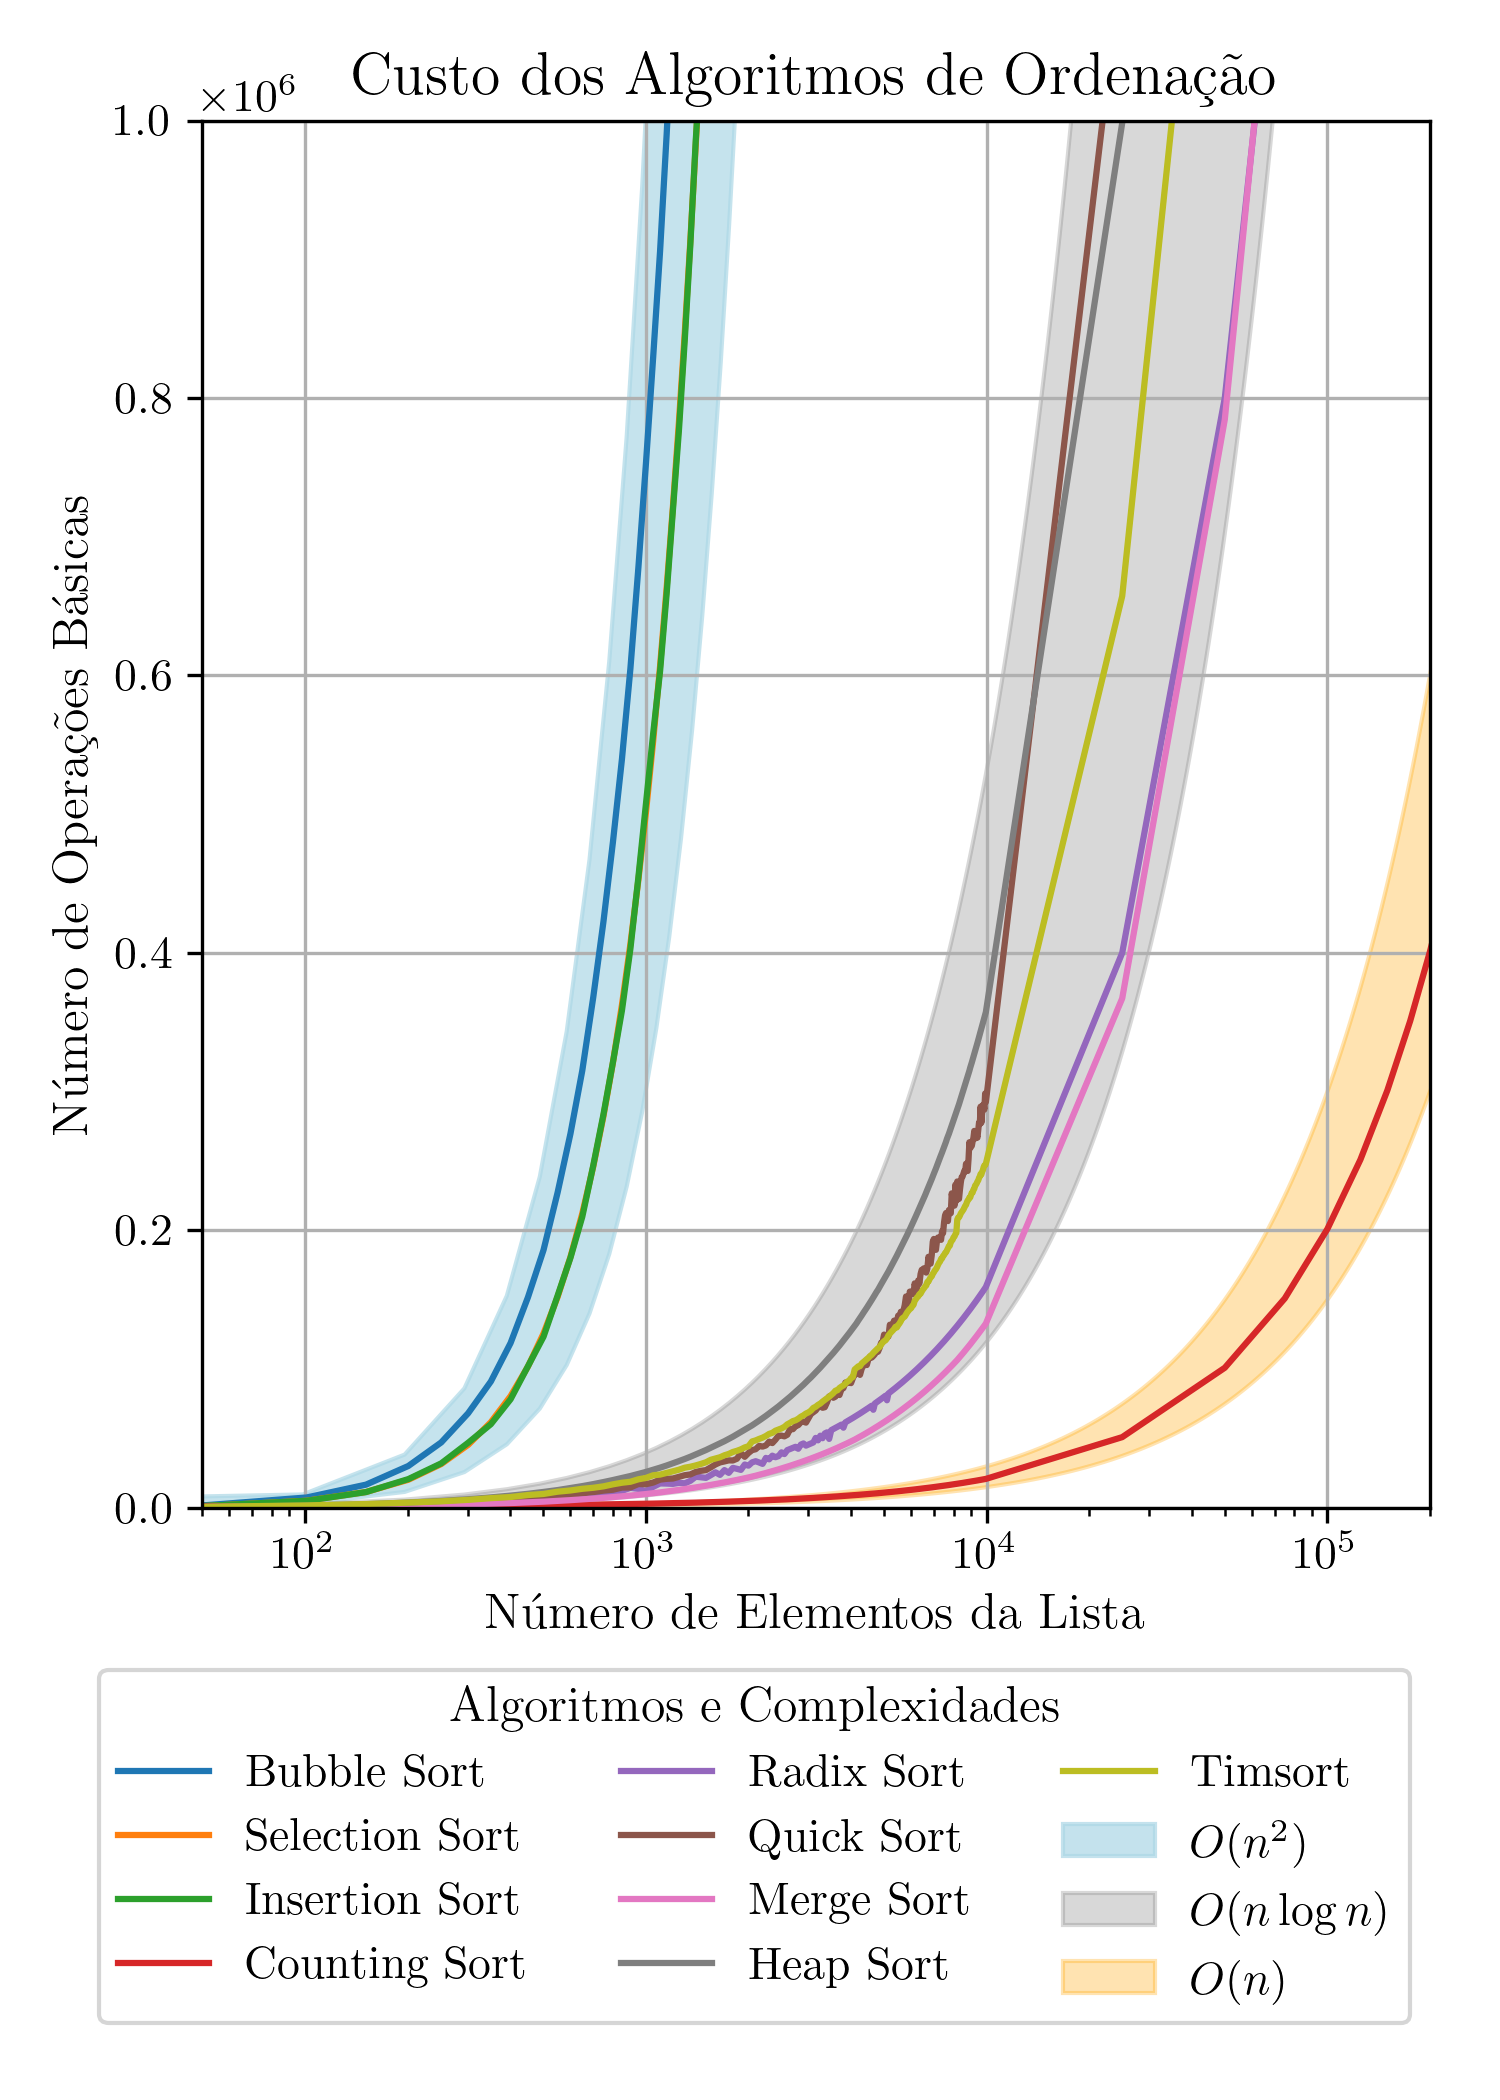
\includegraphics[width=1\linewidth]{sorting_complexities.png}
    \caption{complxidades baseadas no num de ops basicas em listas geradas com numeros inteiros positivos aleatorios até 1000}
    \label{fig:sorting_complexities}
\end{figure}



\bibliographystyle{IEEEtran}
\bibliography{references}

\end{document}



